\sektion{Introduction to Gadsu}

%%%%%%%%%%%%%%%%%%%%%%%%%%%%%%%%%%%%%%%%%%%%%%%%
\fullimageCapt{gadse}{This is a cat.}{8cm}

%%%%%%%%%%%%%%%%%%%%%%%%%%%%%%%%%%%%%%%%%%%%%%%%
\fullimageCapt{ohashi}{This is Shiatsu.}{6.3cm}

%%%%%%%%%%%%%%%%%%%%%%%%%%%%%%%%%%%%%%%%%%%%%%%%
\frame{\frametitle{Gadsu is \ldots} 
\pause
\begin{center}
\begin{Huge}
Gadse
\pause

\vspace{0.5cm}

+ Shiatsu
\pause

\vspace{0.8cm}

= Gadsu
\end{Huge}
\end{center}

}
%%%%%%%%%%%%%%%%%%%%%%%%%%%%%%%%%%%%%%%%%%%%%%%%
\fullimageCapt{gadsu_screenshot}{Visit \href{https://github.com/christophpickl/gadsu}{github.com}}{11cm}

%%%%%%%%%%%%%%%%%%%%%%%%%%%%%%%%%%%%%%%%%%%%%%%%
\frame{\frametitle{Shiatsu is \ldots}

\begin{itemize}
	\item Acpuressure, meridian therapy, physio therapy, massage, stimulation of the nervous system, life coaching
	\item Based on the \textbf{T}raditional \textbf{C}hinese \textbf{M}edicine
	\begin{itemize}
		\item Body and mind seen as a unit, not separated from each other
		\item Concepts like Qi, 5 Elements
	\end{itemize}
\end{itemize}

\begin{figure}[h]
\centering
  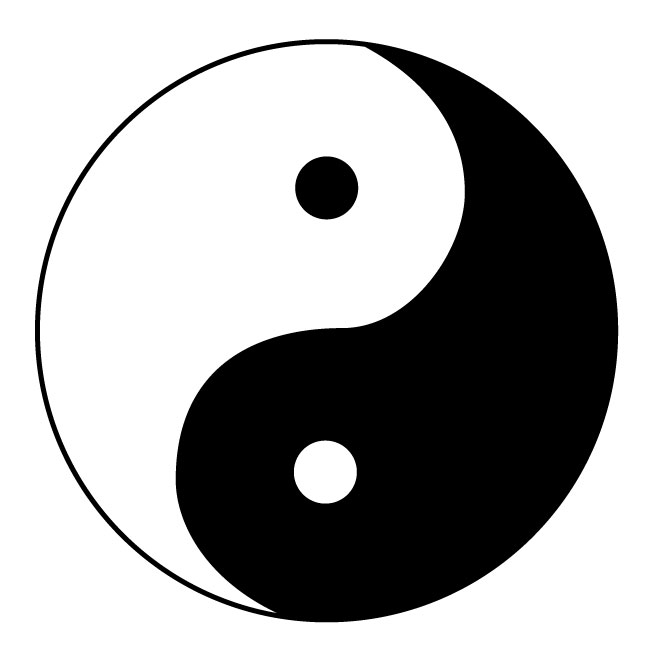
\includegraphics[height=2.0cm]{yinyang}
\end{figure}
}

%%%%%%%%%%%%%%%%%%%%%%%%%%%%%%%%%%%%%%%%%%%%%%%%
\begin{frame}[t]
\frametitle{Features}
\begin{columns}[t]
\begin{column}{0.5\textwidth}
	Present:
	\begin{itemize}
		\item Manage clients, appointments, diagnosis and treatments
		\item Manage medical record
		\item Reporting
		\item GMail integration
		\item Google Calendar integration
		\item Native executables
		\item Auto update software
		\item Auto backup data
	\end{itemize}
\end{column}
\begin{column}{0.5\textwidth} 
	Future:
	\begin{itemize}
		\item TCM assistant
		\item Statistics
		\item Pain indicator
		\item 5 Element widget
		\item Invoicing
		\item Doodle integration
		\item Search / sort clients
	\end{itemize}
\end{column}
\end{columns}
\end{frame}

%%%%%%%%%%%%%%%%%%%%%%%%%%%%%%%%%%%%%%%%%%%%%%%%
\begin{frame}
\frametitle{Technology Stack}
\begin{itemize}
	\item Gradle
	\item Swing
	\item Guice
	\item Spring JDBC
	\item HSQLDB + Flyway
	\item Jasper, Pdfbox
	\item Freemarker
	\item TestNG, Mockito, Hamcrest
	\item UISpec4J
\end{itemize}

\end{frame}
